\documentclass[12pt]{article}
\usepackage{amsmath}
\usepackage{amssymb}
\usepackage{graphicx}
\usepackage{caption}

% Setup
\captionsetup{font={small}}

\title{Bayes Theorem: A Geometric Interpretation} 
\author{Adam Cuculich} 
\date{November 24, 2023}

\begin{document}

\maketitle % This command prints the title

\subsection*{Introduction:}
This document aims to provide a geometric, or visual, interpretation of Bayes’ Theorem. It endeavors to guide readers from the fundamental principles to an intuitive understanding of the theorem. Starting with known probabilities, the paper derives Bayes’ Rule using conditional probabilities and advances to a pragmatic application of Bayes’ Theorem, addressing probability distributions represented as random variables. In doing so, I strive to bridge analytical descriptions with geometric interpretations, thus offering a comprehensive insight into the theorem’s intrinsic dynamics. Ultimately, the goal is to lay down a theoretical yet intuitive foundation in Bayesian statistics. \\\\

\newpage

\subsection*{Bayes Rule}
Shown below, Bayes' Rule can be derived using known conditional probabilities. A geometric interpretation of the underlying mechanics is also provided in this section.
\subsubsection*{Conditional Probabilities:}
Let \(A\) and \(B\) be distinct sets of events in set \(S\), where \(S\) is the sample space of all possible events. Set theoretically, let  \( A \subseteq S \) and \( B \subseteq S \). \\\\
The conditional probability of event \( A \), given event \( B \) is defined as:
\begin{equation}
P(A \mid B) = \frac{P(A \cap B)}{P(B)}
\end{equation}

\noindent This relationship can be expressed visually as follows:\\

% Image
\begin{figure}[h!]
\centering
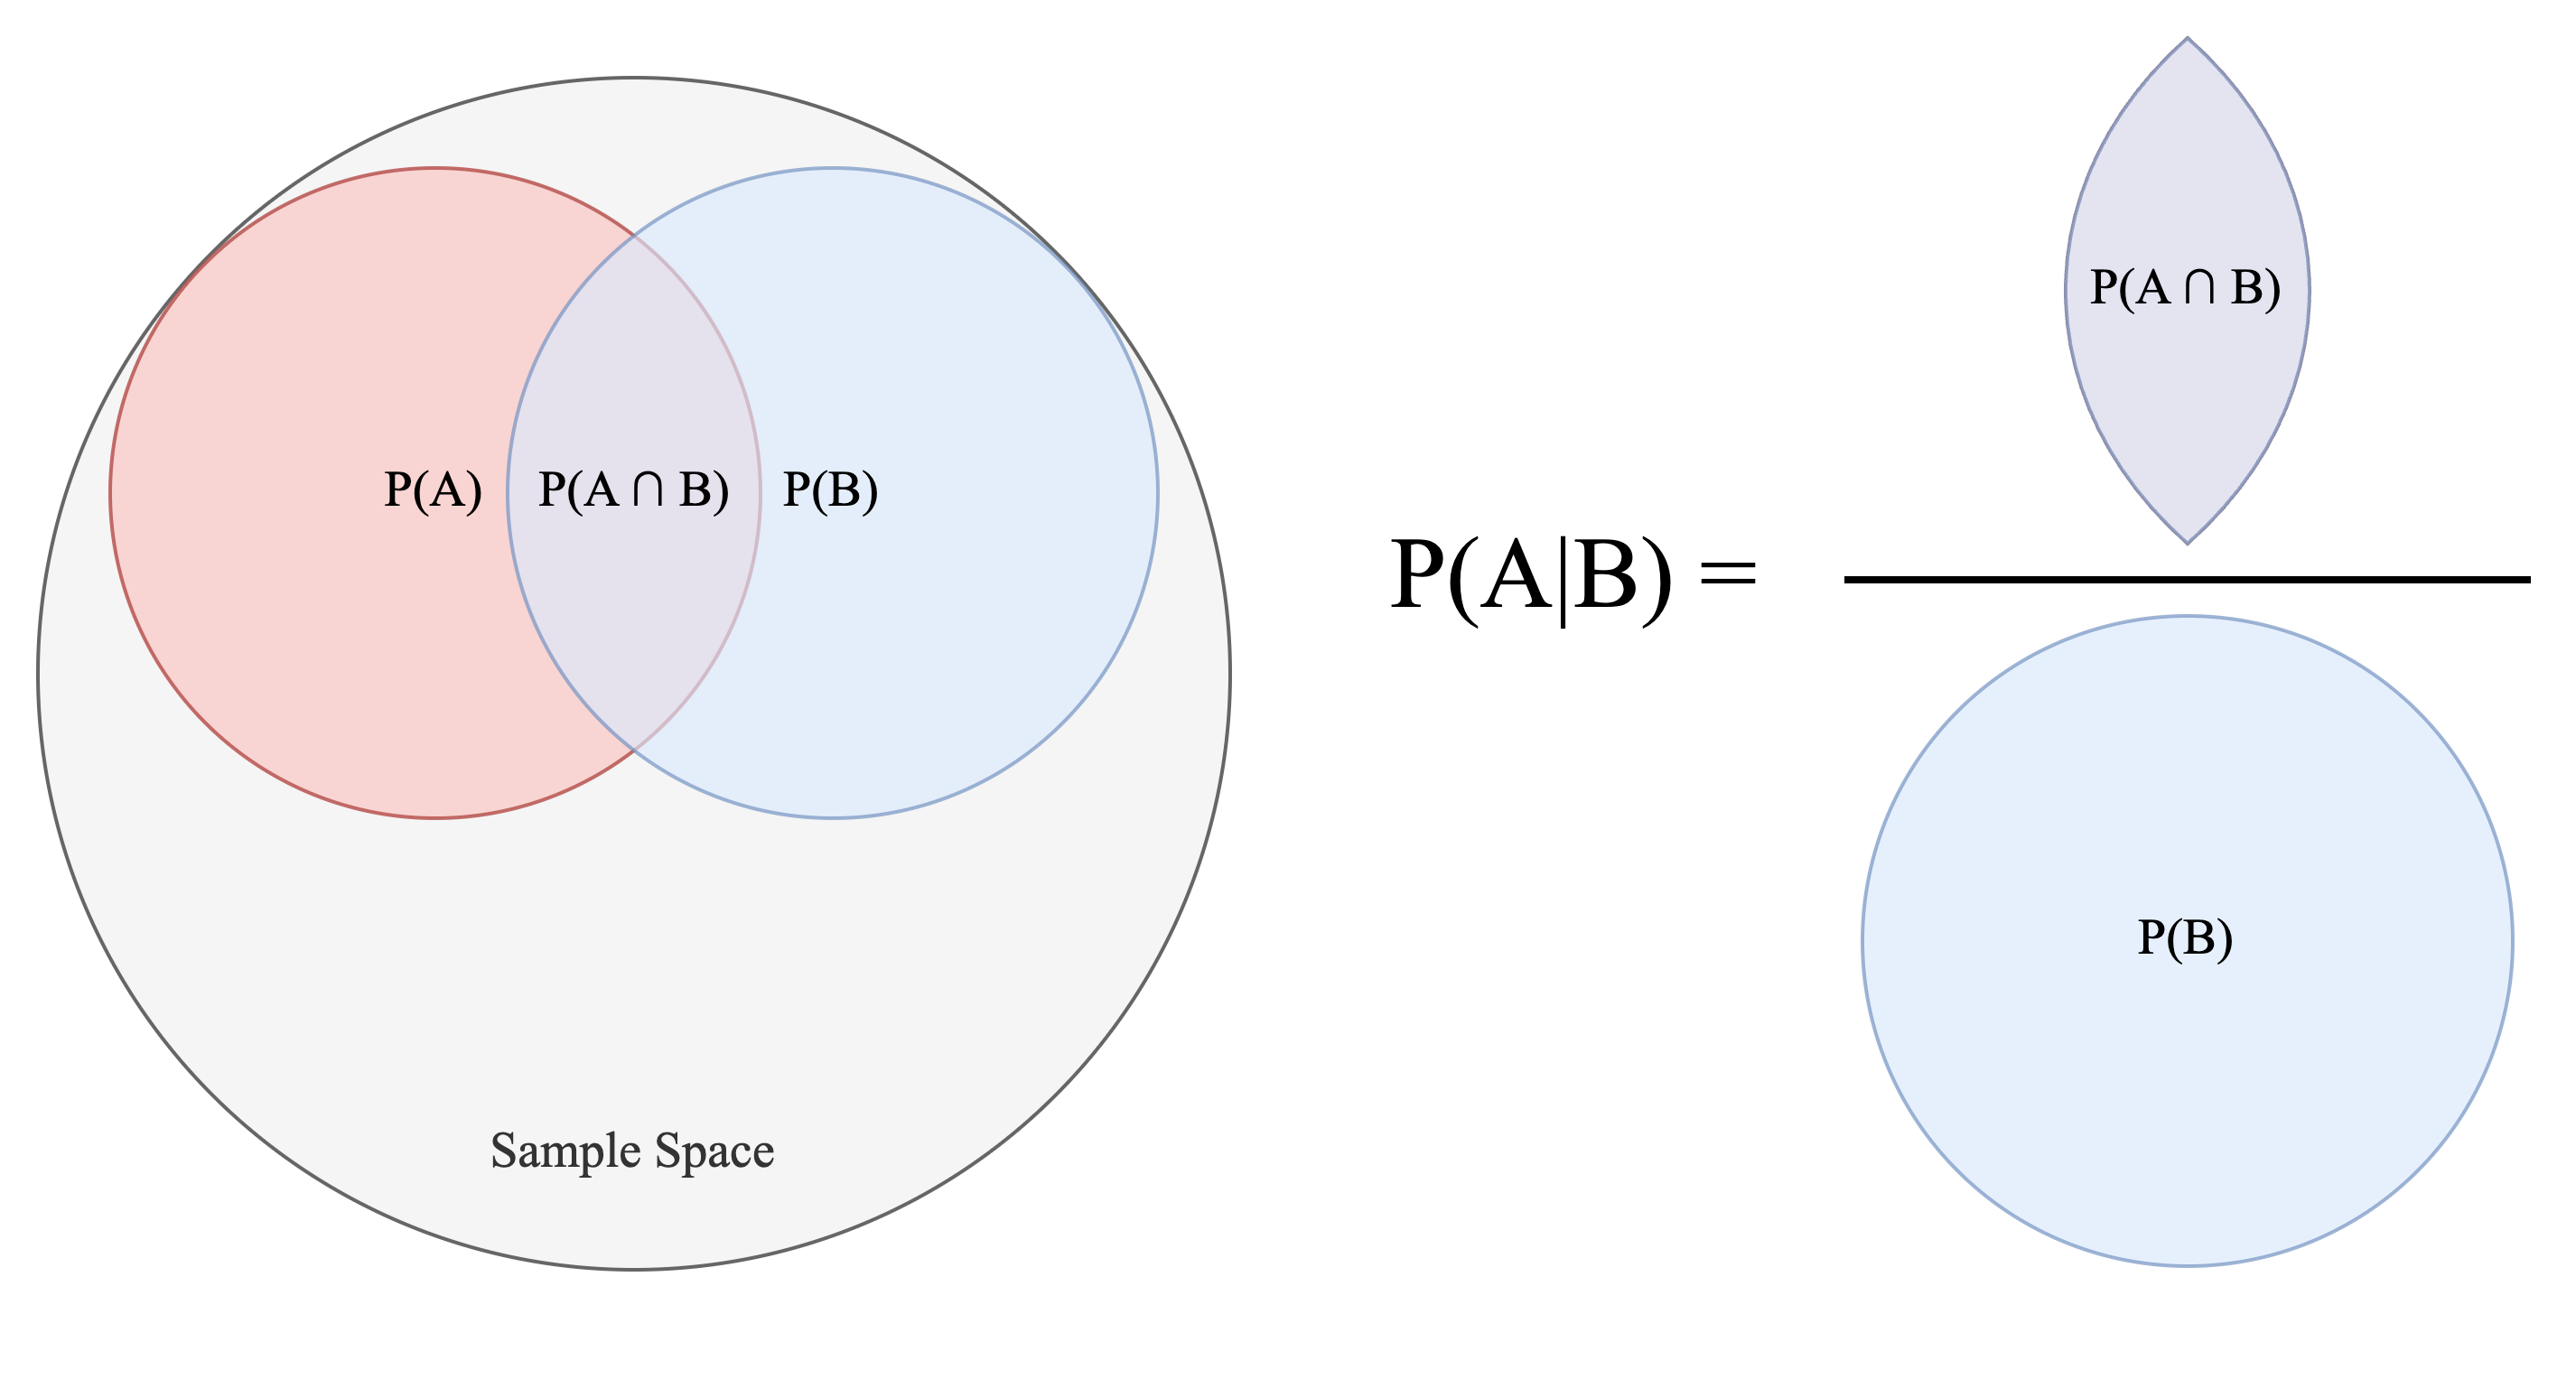
\includegraphics[width=1.0\textwidth]{assets/visual_1.png} 
\caption{A visual representation of conditional probability}
\label{fig:cond_prob}
\end{figure}

\noindent Shown above, some of the shapes are subsets of other shapes. Each shape represents an event, or set of outcomes, that an outcome can be categorized as. Each shape’s area is used to represent the probability of an outcome being categorized into the event the shape represents. The sample space $S$ represents all possible events relevant to a specific, given context. Because all possible, mutually exclusive and collectively exhaustive events are encompassed within $S$, you can be 100\% certain that an outcome will be categorized within the set of outcomes that is $S$. Therefore, $P(S) = 1$. As a useful representation, the probability of an outcome being categorized as a particular event is a number that describes the certainty of that outcome taking on the specific properties that define that event. When it comes to conditional probabilities, the following question provides insight into their nature: “given you know $B$ happened, what’s the probability $A$ also happened?” The added knowledge of $B$’s occurrence confines the set of outcomes to those in $B$. Succinctly, $P(A \mid B)$ is the proportion of occurrences of B where A also occurs. This proportion can be 0, 1, or anywhere in between. For example, if events $A$ and $B$ are mutually exclusive, then the probability that $A$ occurs given a known $B$ occurrence would be 0. If instead, $A$ always occurs when $B$ occurs, it would be 1.	

\subsubsection*{Deriving Bayes' Rule:}
Given the definition of conditional probability,
\begin{equation}
P(A \mid B) = \frac{P(A \cap B)}{P(B)}
\end{equation}
Similarly, \\
\begin{equation}
P(B \mid A) = \frac{P(B \cap A)}{P(A)}
\end{equation}
By equivalence, \\
\begin{equation}
P(A \cap B) = P(B \cap A)
\end{equation}
\begin{equation}
P(A \cap B) = P(A \mid B) P(B)
\end{equation}
\begin{equation}
P(B \cap A) = P(B \mid A) P(A)
\end{equation}
\begin{equation}
P(A \mid B) P(B) = P(B \mid A) P(A)
\end{equation} \\

\noindent Hence, Bayes' Rule is given by:
\begin{equation}
P(A \mid B) = \frac{P(B \mid A) P(A)}{P(B)}
\end{equation}

\noindent With Bayes' Rule established, we transition from the abstract events, A and B, to the concepts of experimentally observed events (Evidence, E) and proposed hypotheses (H). This transition is underpinned by the principle that, akin to A and B, both observed data (evidence) and hypotheses are events within a shared sample space. Hypotheses are characterized as events that are evaluated in light of the observed data.

\begin{equation}
P(H \mid E) = \frac{P(E \mid H) P(H)}{P(E)}
\end{equation}

\subsubsection*{Total Probability:}
\noindent Above, $P(E)$ is the total probability of the evidence occurring, taking into account all possible, mutually exclusive hypotheses. Now, suppose you constructed an array with all possible hypotheses, each with its own probability. To ensure that all cases and their compliments are accounted for, the sum of all of the hypotheses' probabilities should be 1. For each hypothesis, there will be some probability of the evidence in question occurring, given that hypothesis (a conditional probability). For clarity, here the evidence is conditioned on that hypothesis. We now have an array where each element in that array is a conditional probability: namely, probability of the evidence, E, given that element's hypothesis. This can be expressed for $n$ hypotheses as follows:

\begin{equation}
P(E) = P(E \mid H_1) P(H_1) + P(E \mid H_2) P(H_2) + ... + P(E \mid H_n) P(H_n)
\end{equation}

\noindent Or more succinctly, 

\begin{equation}
P(E) = \sum_{i=1}^{n} P(E \mid H_i) P(H_i)
\end{equation}

\noindent With this established, Bayes' Rule can be expressed as follows for a given hypothesis, $H_j$: 

\begin{equation}
P(H_j \mid E) = \frac{P(E \mid H_j) P(H_j)}{\sum_{i=1}^{n} P(E \mid H_i) P(H_i)}, \text{ where } j \in \{1, 2, \ldots, n\}
\end{equation}

\subsection*{Bayes' Rule: A Geometric Interpretation:}
\noindent The foregoing states that the probability of a hypothesis, given evidence is the conditional probability of evidence given that particular hypothesis ($H_j$) over the total probability of the evidence, taking into account all possible hypotheses. This can be visually represented as follows: \\

% Image
\begin{figure}[h!]
\centering
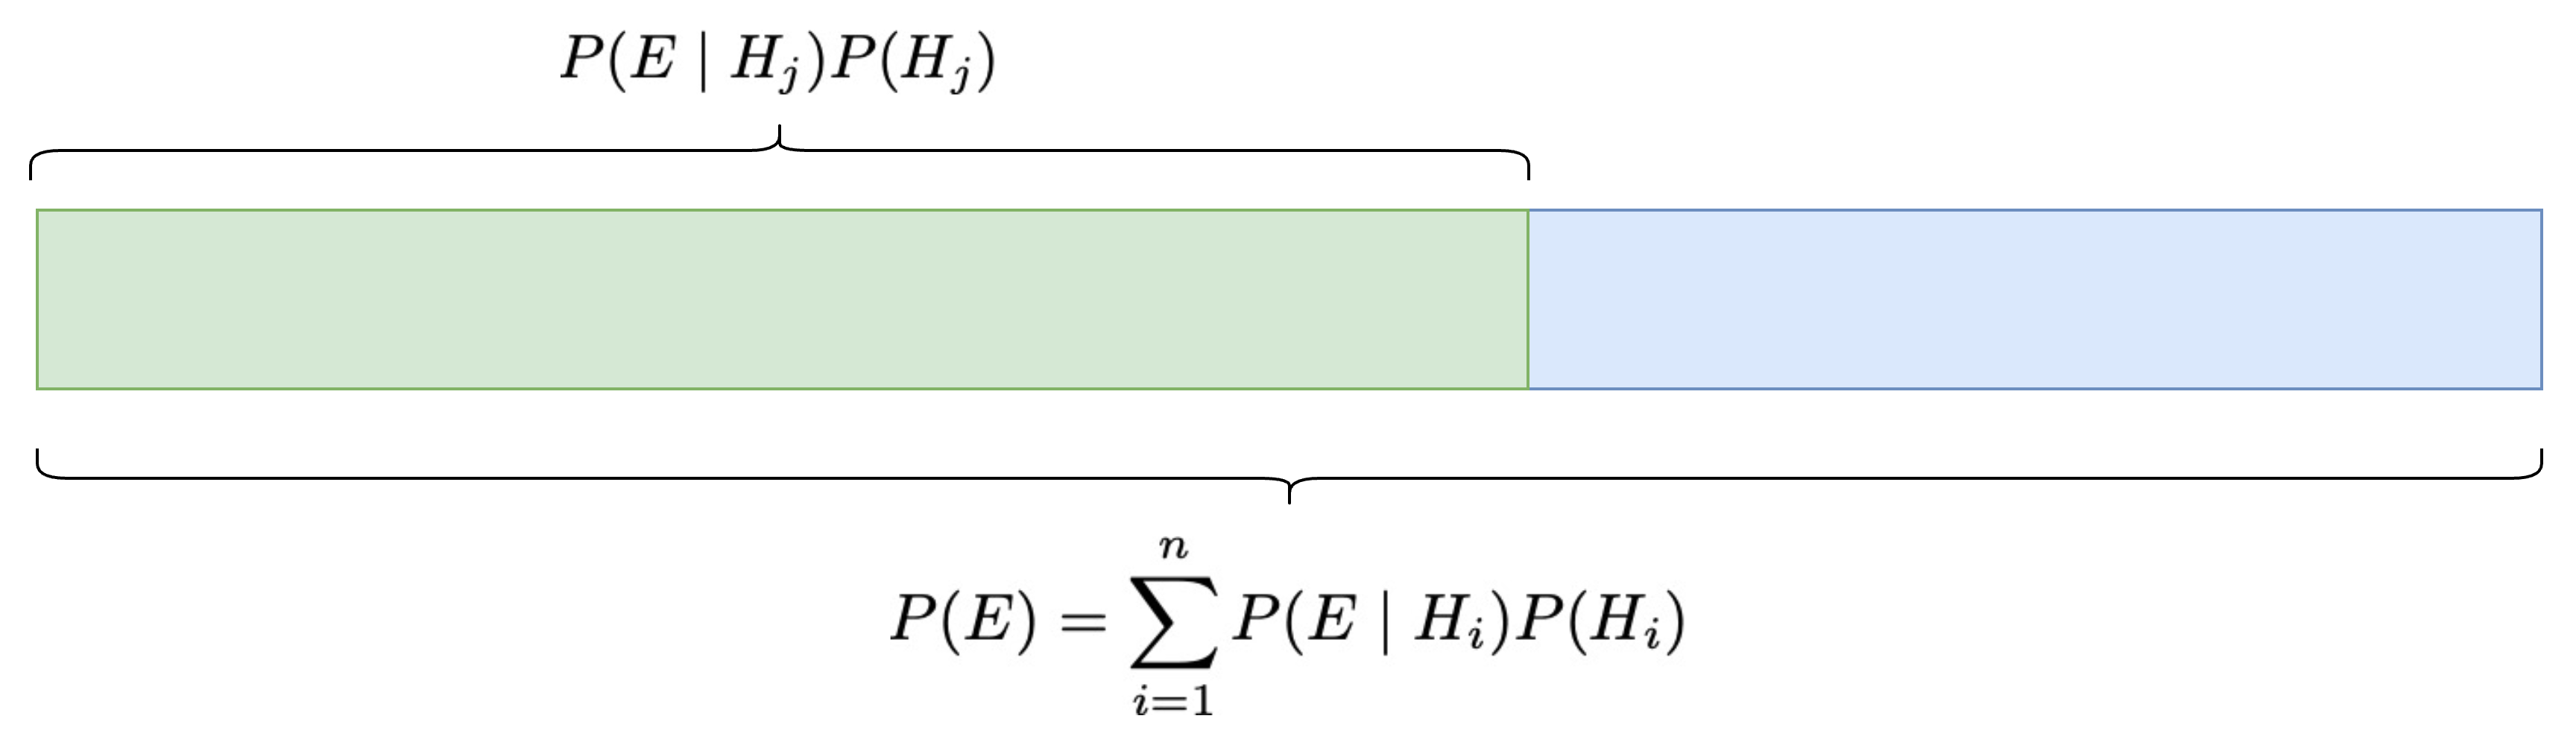
\includegraphics[width=0.75\textwidth]{assets/visual_2.png} 
\caption{A visual representation of Bayes' Rule}
\label{fig:cond_prob}
\end{figure}

\noindent Now, let's lay the ground work for a geometric interpretation. Bayes' Rule can be rearranged as follows:\\

\noindent Given:
\begin{equation}
P(E \mid H) = \frac{P(E \cap H)}{P(H)},
\end{equation}

\noindent Substituting this for all occurrences in equation 12, it can be shown that:

\begin{equation}
P(H_j \mid E) = \frac{P(E \cap H_j)}{\sum_{i=1}^{n} P(E \cap H_i)}, \text{ where } j \in \{1, 2, \ldots, n\}
\end{equation} \\

\noindent This states that probability of hypothesis $H_j$, given evidence, E,  is the intersection of the evidence with $H_j$ over the sum of all intersections between E and all hypotheses. As a visual demonstration, take the case where there are 4 hypotheses.

\newpage

\noindent Suppose a hypothesis-evidence space, in which the x-axis represents all possible hypotheses and their probabilities, and the y-axis represents the probability space for evidence conditioned on a given hypothesis.

\begin{figure}[h!]
    \centering
    \begin{minipage}{0.50\textwidth}
        \centering
        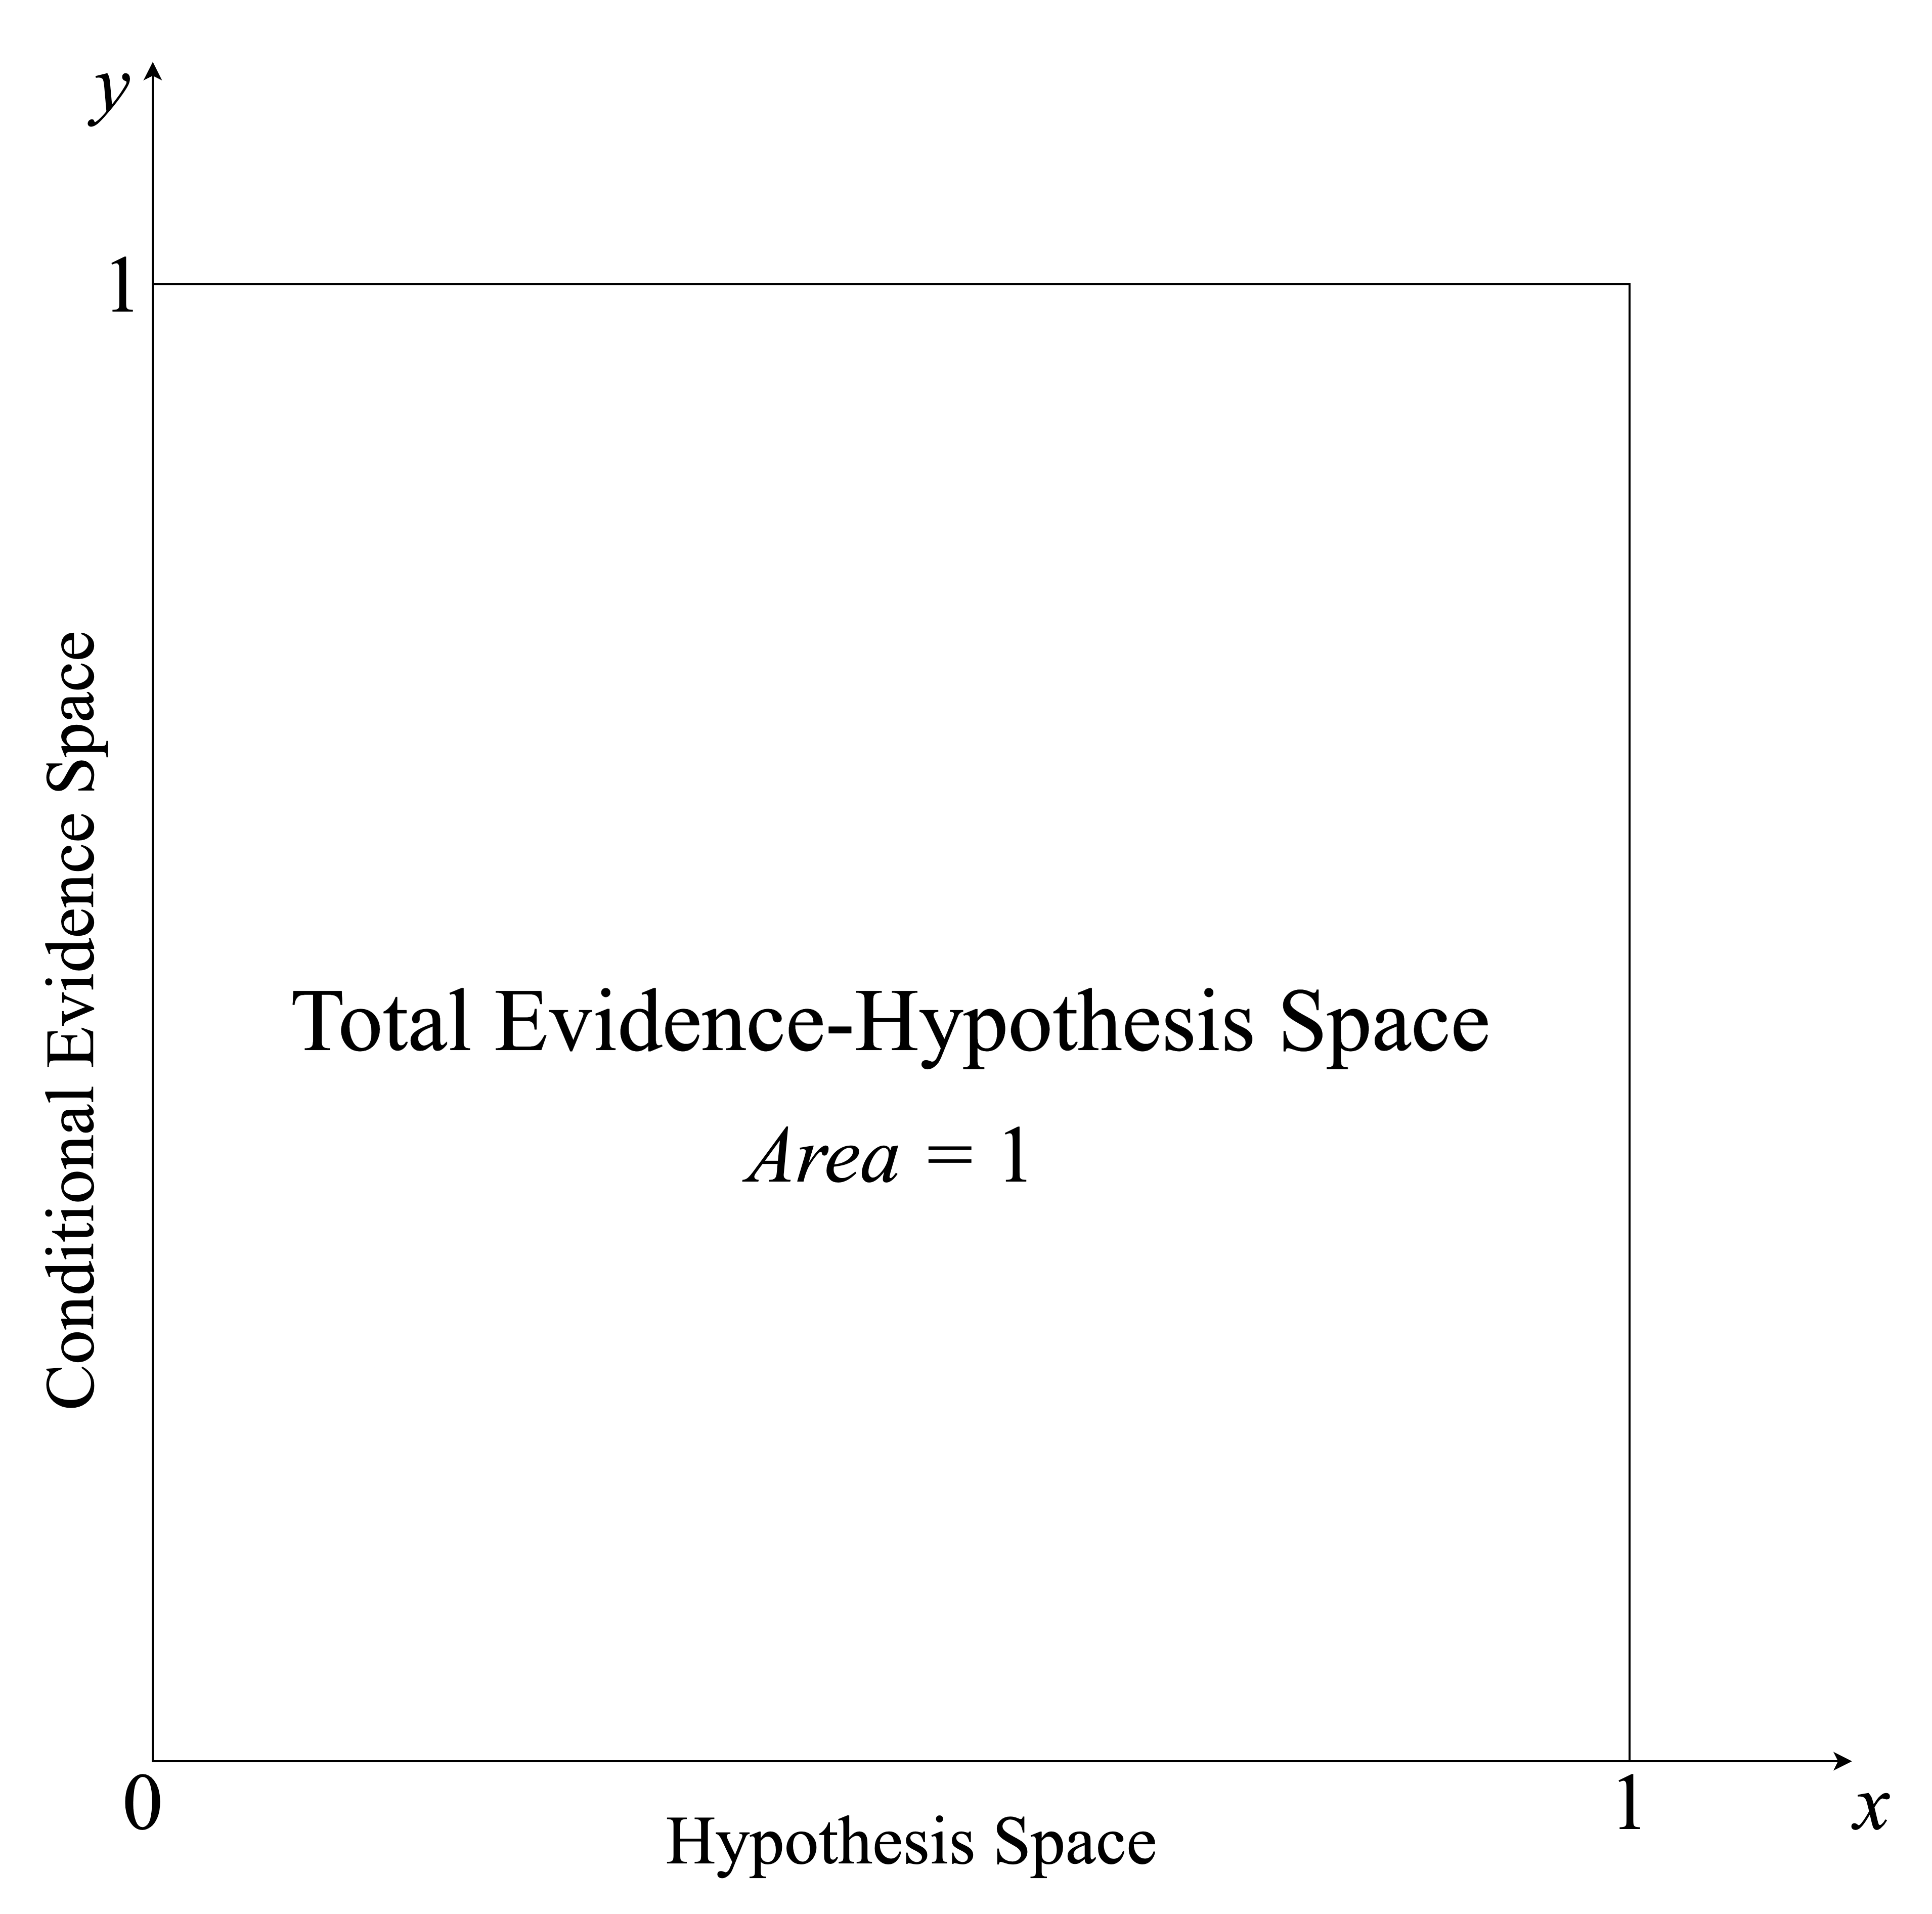
\includegraphics[width=\textwidth]{assets/visual_3.png}
    \end{minipage}\hfill
    \begin{minipage}{0.50\textwidth}
        \centering
        \includegraphics[width=\textwidth]{assets/visual_4.png}
    \end{minipage}
    \caption{The hypothesis-evidence space divided by hypotheses.}
    \label{fig:both_visuals_3_4}
\end{figure}


\noindent Shown above, the hypothesis space can be divided into all relevant hypotheses, denoted by the subsections above.

\newpage

\noindent Each hypothesis will have its own probability of evidence, previously referenced as $P(E \mid H_i)$ in the equation 11 above. These conditional probabilities can be represented as the y-axis component of the joint probability sections below.

\begin{figure}[h!]
    \centering
    \begin{minipage}{0.72\textwidth}
        \centering
        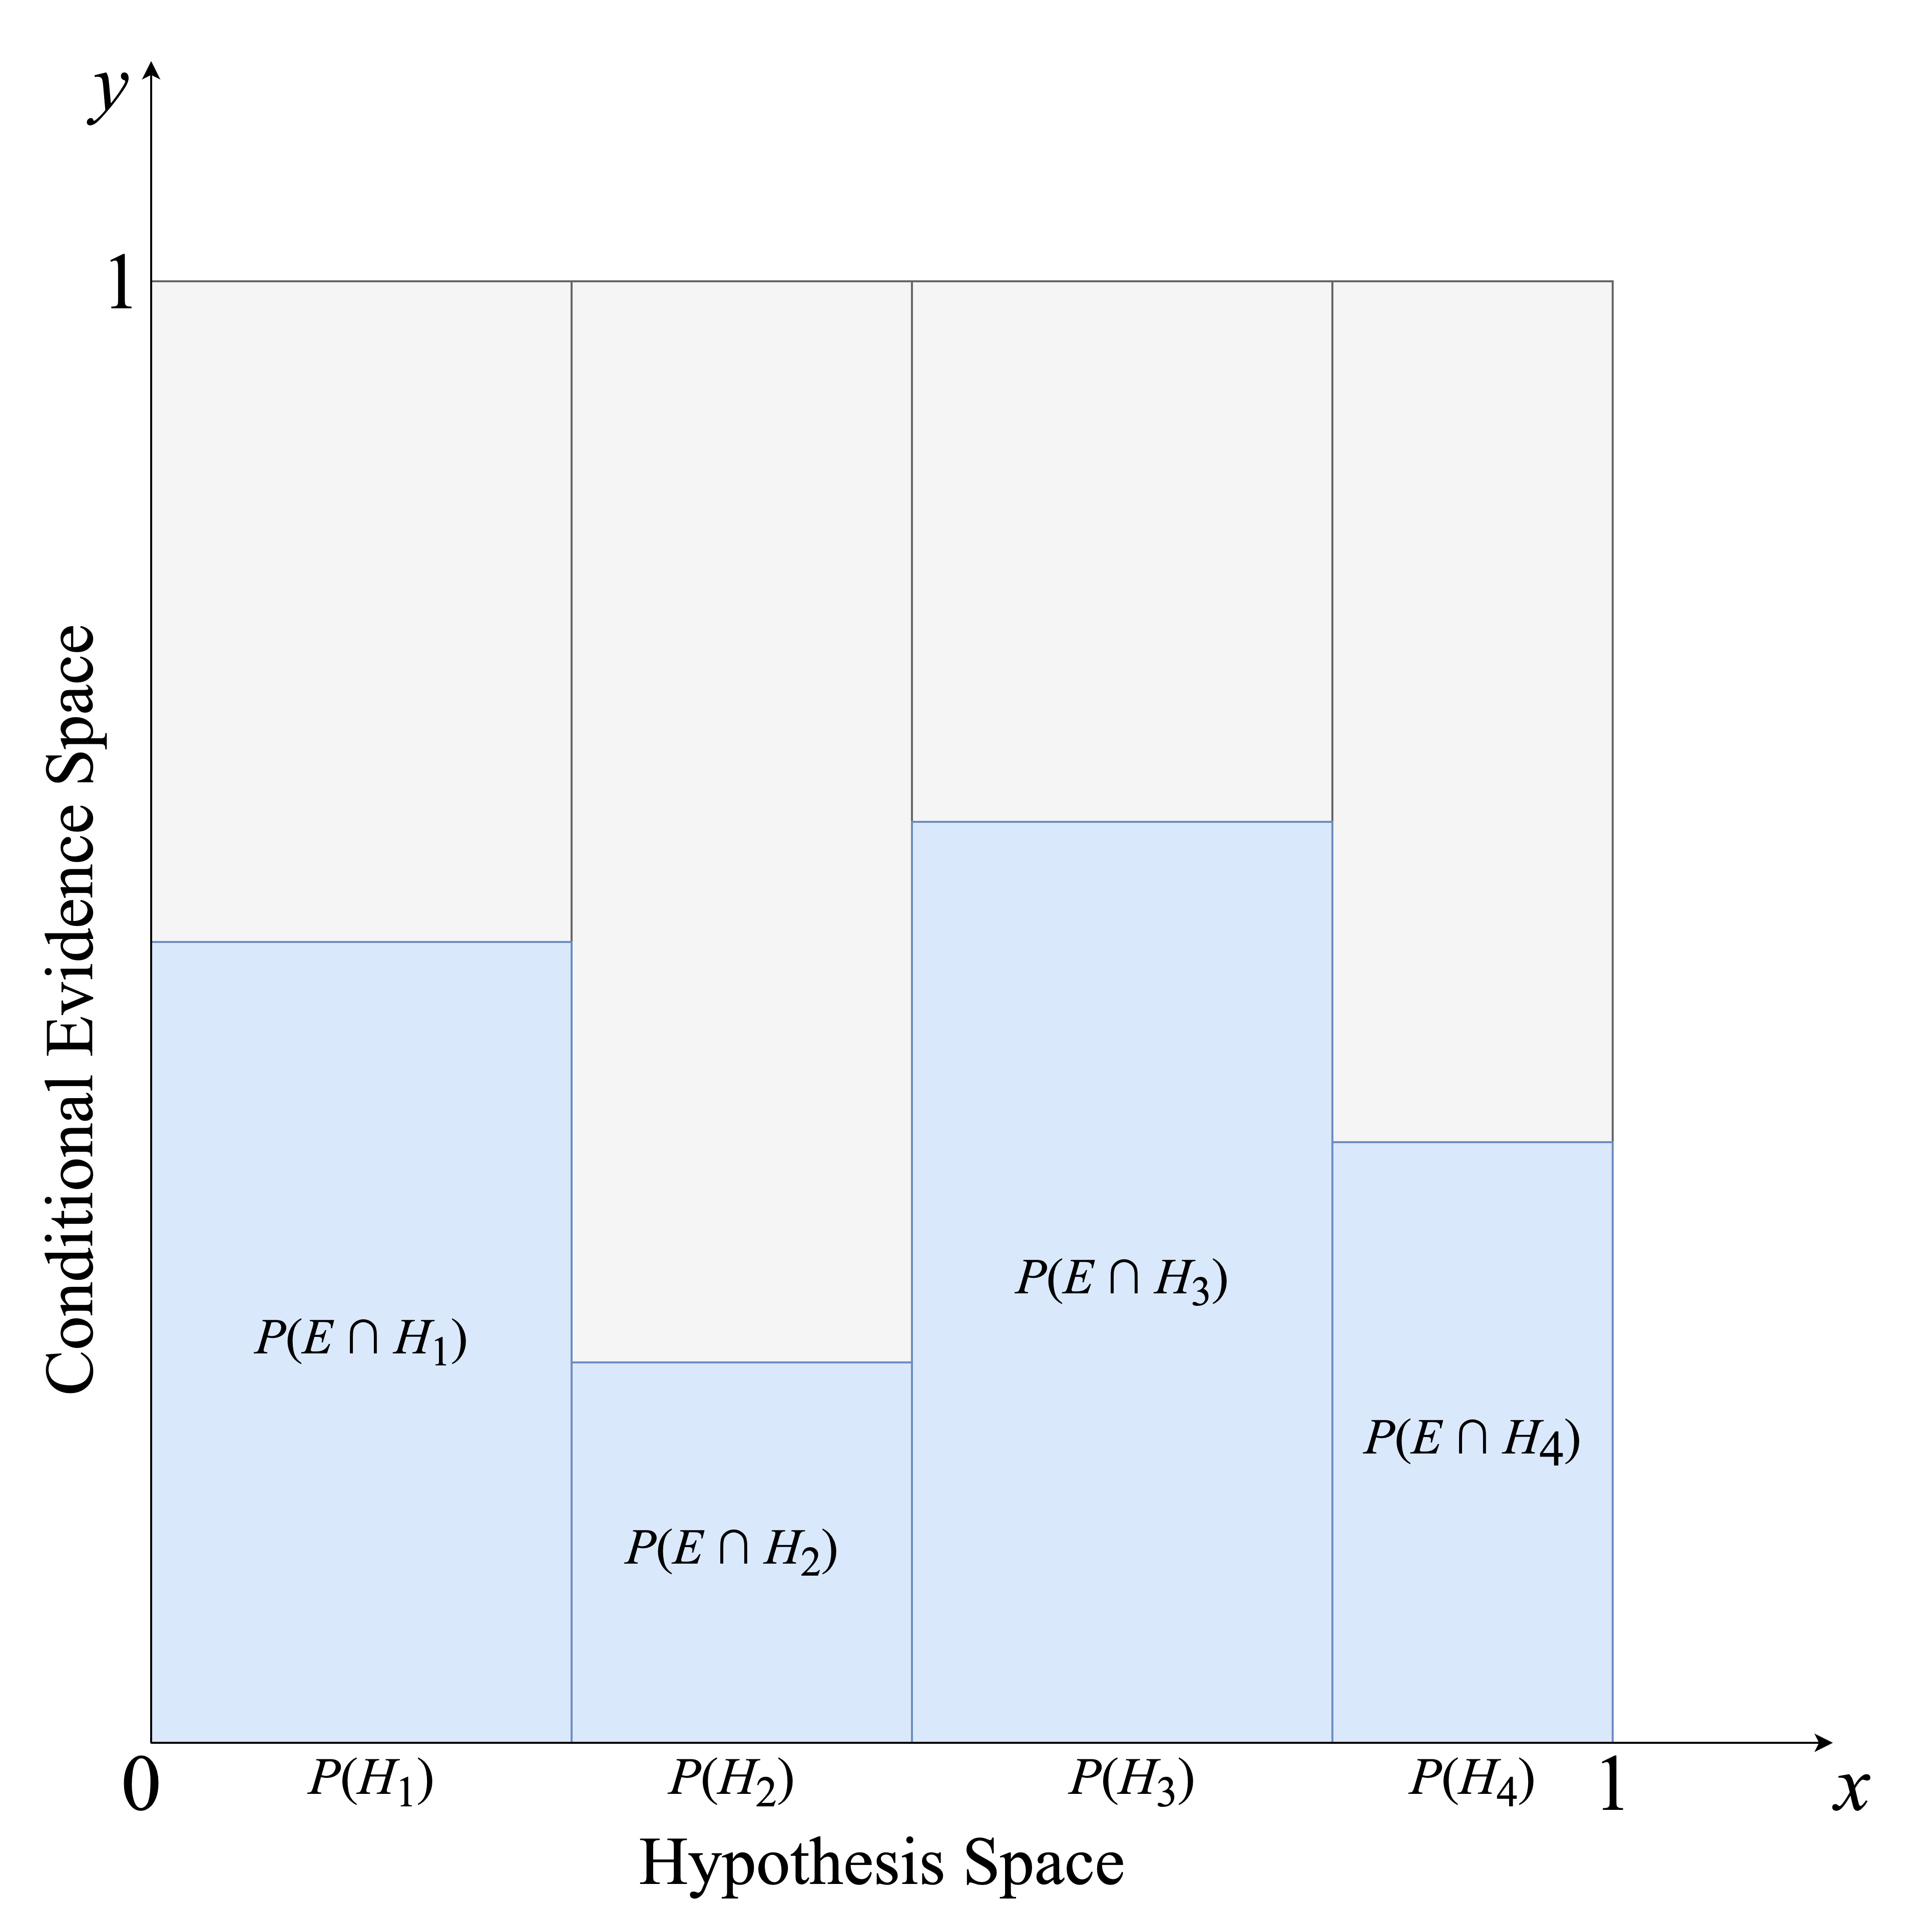
\includegraphics[width=\textwidth]{assets/visual_5.png}
    \end{minipage}\hfill
    \begin{minipage}{0.28\textwidth}
        \centering
        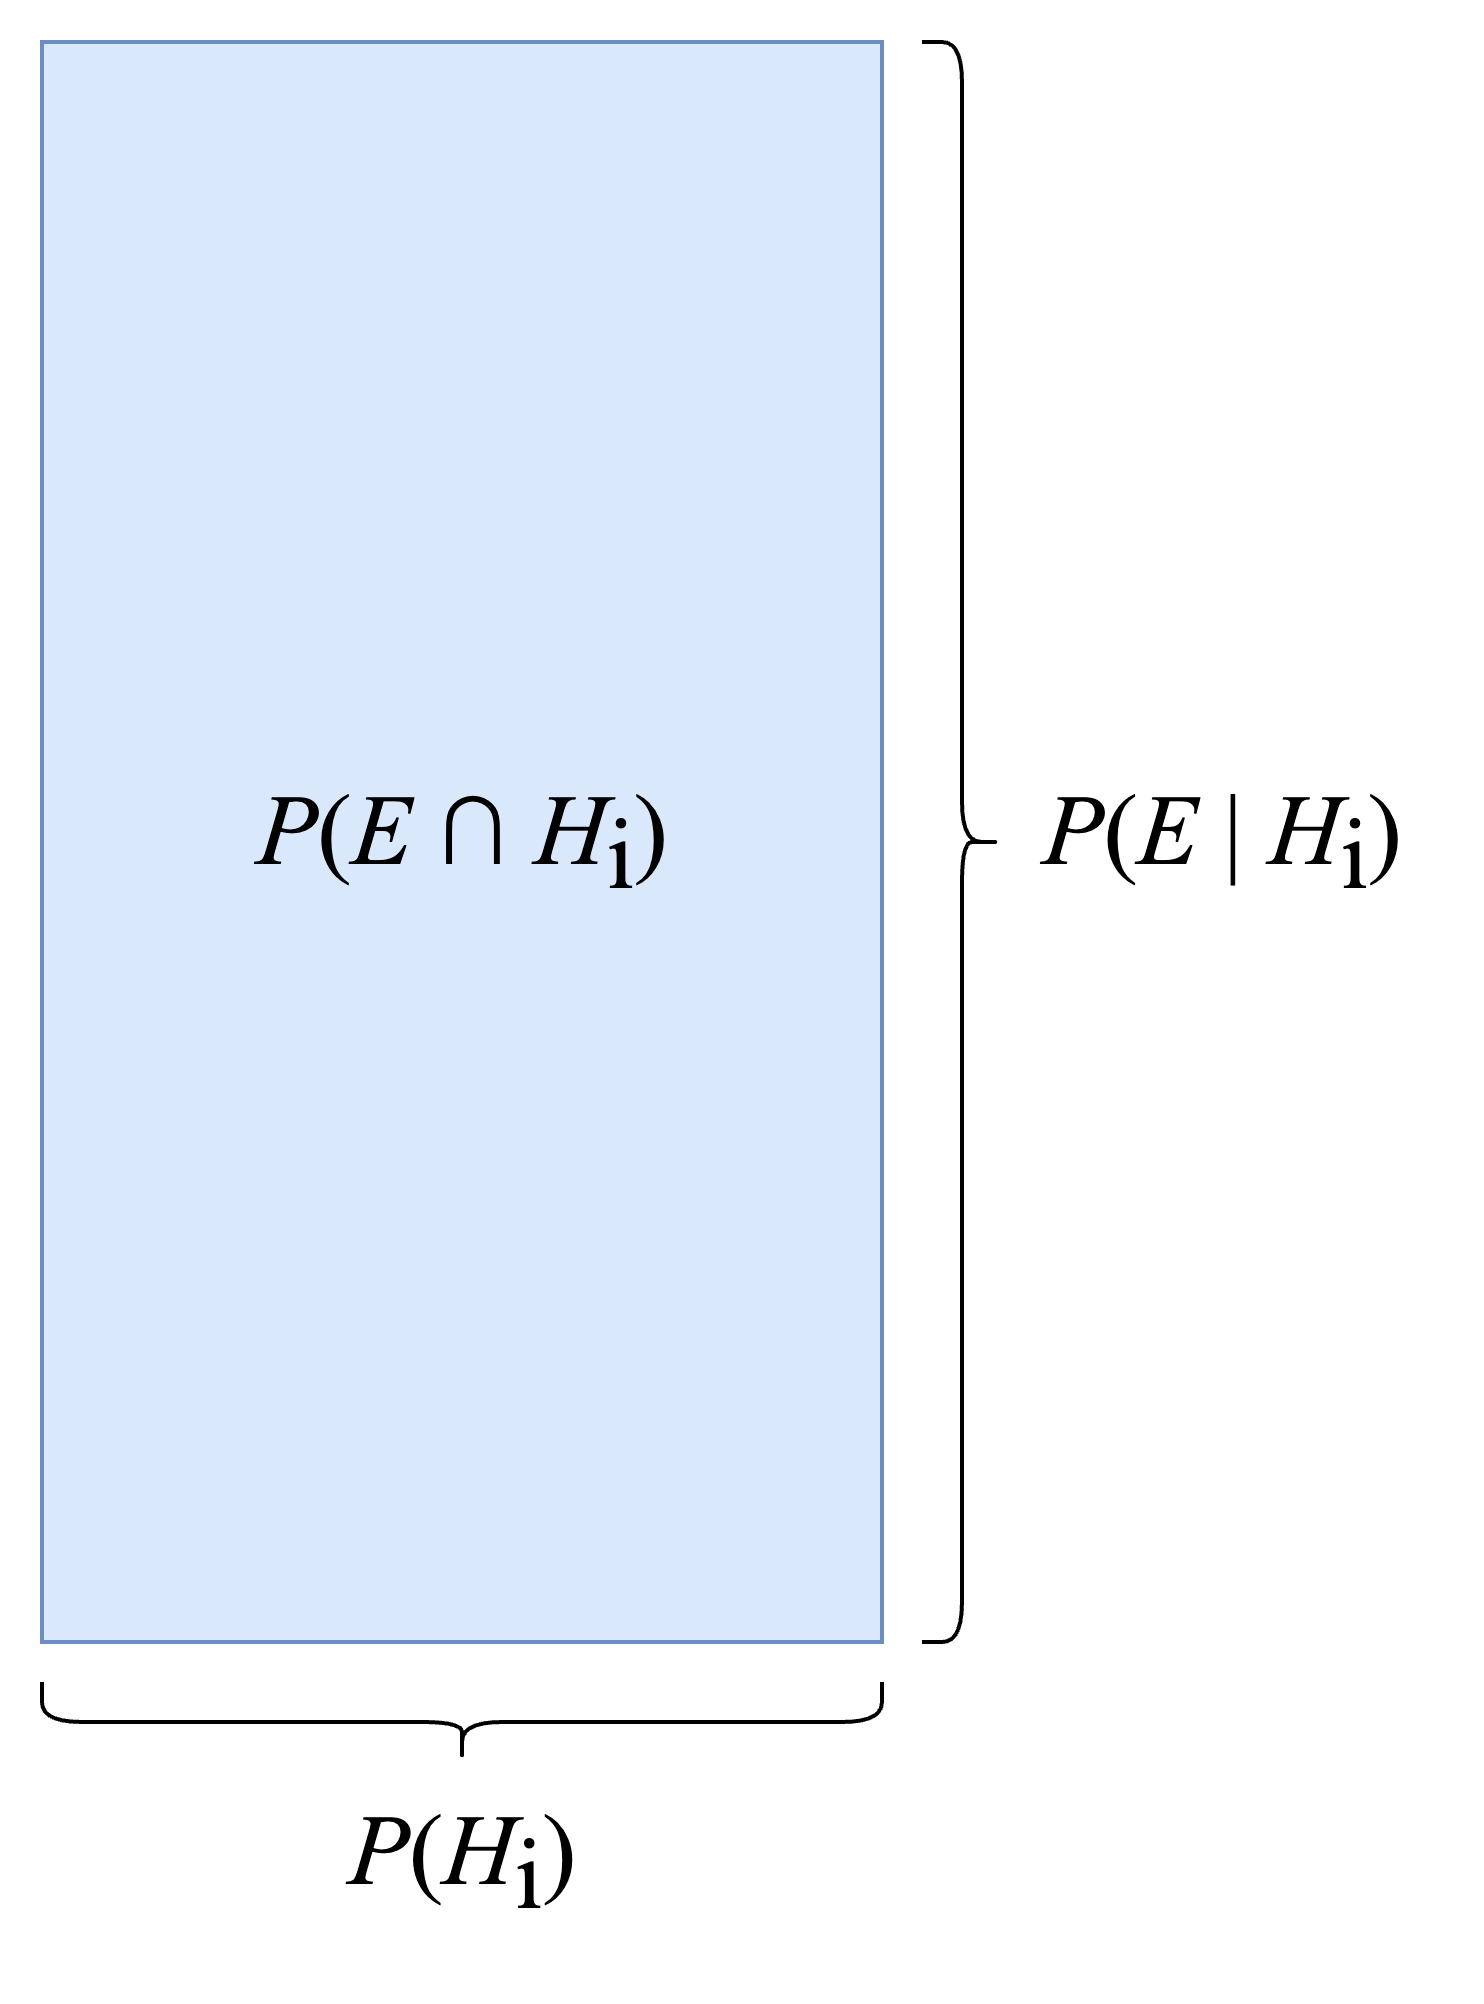
\includegraphics[width=\textwidth]{assets/visual_6.png}
    \end{minipage}
    \caption{Left: Hypothesis-evidence intersections visualized}
    \label{fig:both_visuals}
\end{figure}

\noindent Examining a single, arbitrarily-chosen subsection, note that the subsection's area is equal to the probability of the hypothesis multiplied by the probability of evidence, given that specific hypothesis. This finding is consistent with equation 5 above.

% Image
\begin{figure}[h!]
\centering
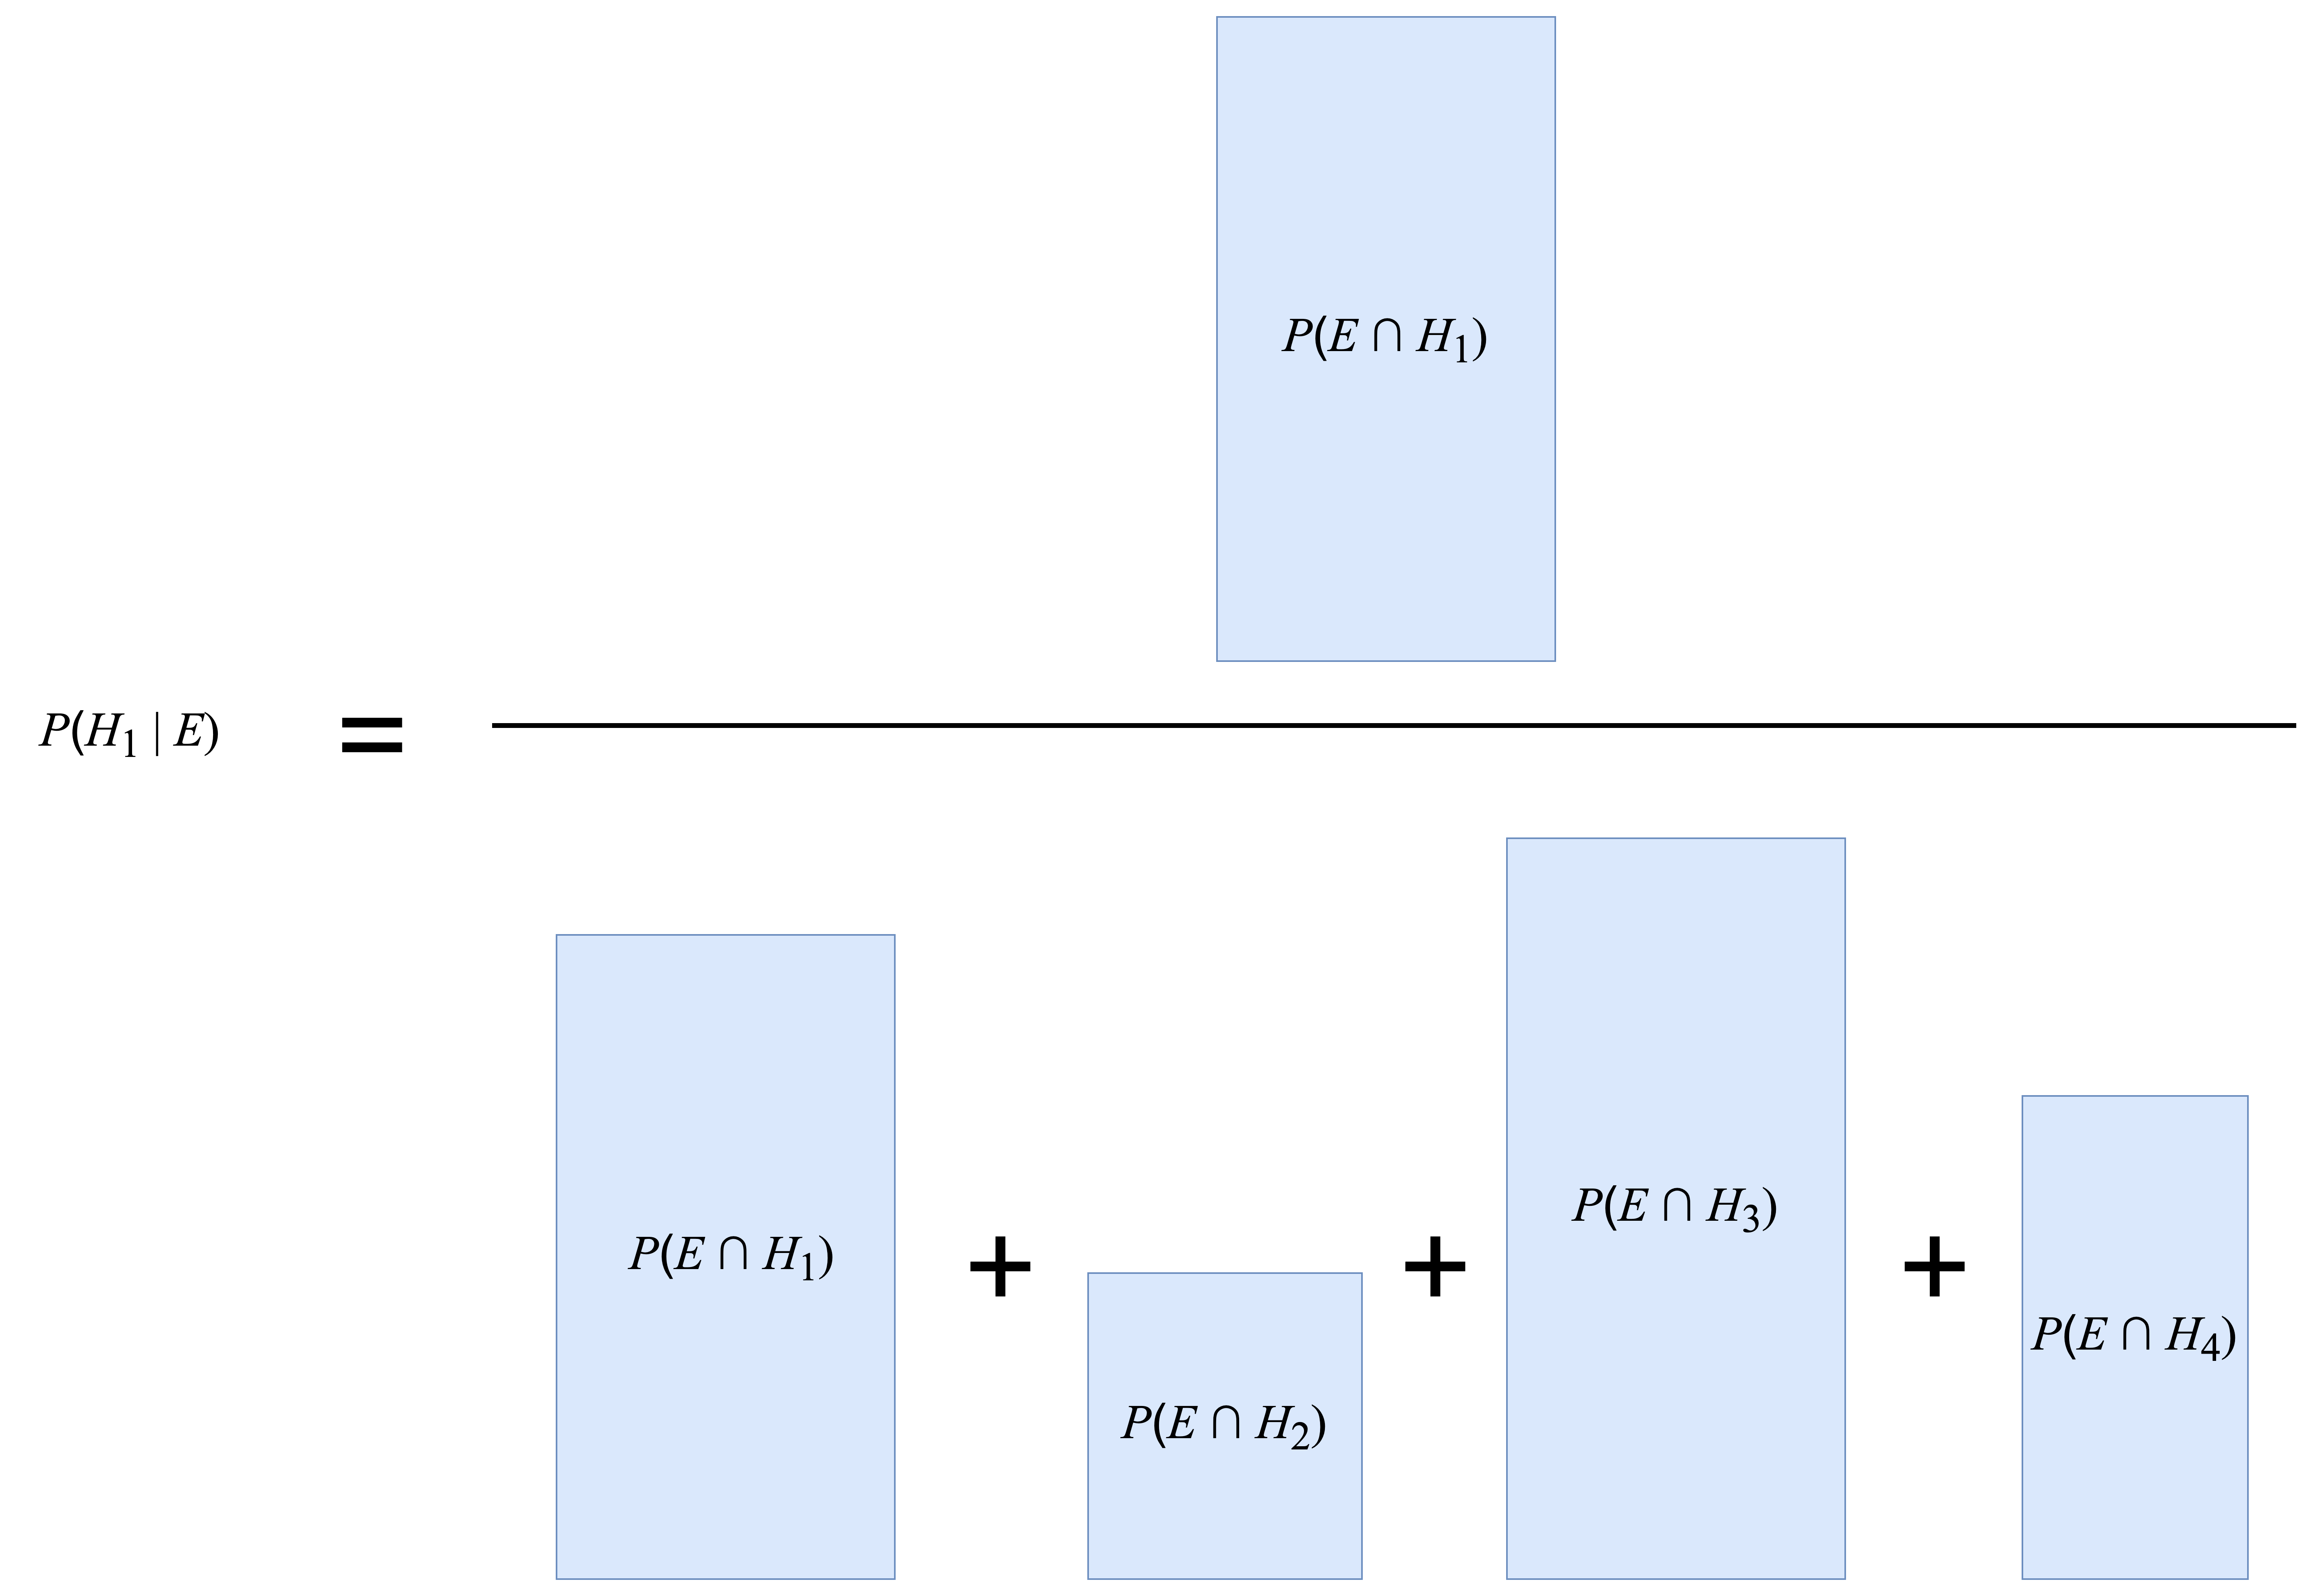
\includegraphics[width=1.0\textwidth]{assets/visual_7.png} 
\caption{Probability of first hypothesis given evidence, visualized.}
\label{fig:cond_prob}
\end{figure}

\newpage

\subsection*{Bayes' Theorem with Continuous Random Variables:}
\noindent The above presupposes that the probabilities involved in Bayes' Rule are known. In the real world, however, probabilities may not be known with certainty. To deal with such cases, the same mechanics can be applied with random variables. To mathematically express the uncertainty of such variables, we use probability distributions in place of known probabilities. Such probability distributions are what's meant by the term, "random variables". Using random variables, Bayes' Theorem is expressed as:

\begin{equation}
\pi(\theta \mid x) = \frac{f(x \mid \theta) \pi(\theta)}{\int_{\Theta} f(x \mid \theta) \pi(\theta) d\theta}
\end{equation}

\noindent It's worth taking some time to understand what this equation is expressing. Intuitively, we know that Bayes' Theorem incorporates information from both experiment and prior beliefs, but to what end? We've heard that a bayesian update is the process by which a prior distribution is updated to a posterior distribution in light of experimental evidence, but how exactly is that achieved? In an effort to gain a deeper understanding, let's first understand the numerator of the theorem, as the denominator is simply the integral of the numerator with respect to $\theta$. \\

\subsection*{Likelihood}
\noindent The term, $f(x\mid\theta)$, is often referred to as the likelihood. Here, the likelihood function evaluates the plausibility of the data $x$ under a statistical model parameterized by $\theta$, and identifies the parameter values that are most probable given the observed data. This definition involves some 'statistical model', about which the data plausibility can be assessed against.

\paragraph{Model Selection}
Let's piece these concepts together with an example. Suppose that we're modeling the 'time to an event', say, the operating lifetime of a certain type of component in a machine. Also, suppose that we have reason to believe the lifetime of that component can be modeled as an exponential distribution:

\begin{equation}
f(x \mid \theta) = \theta e^{-\theta x}, \text{ where } \theta > 0 \text{ and } x \ge 0
\end{equation}

\noindent Here, $f(x \mid \theta)$ is a function of $x$ and $\theta$, where $\theta$ is the rate parameter. The greater the value of $\theta$, the faster the function decays toward 0. At this point, we've proposed a statistical model as an attempt to explain the lifetime of the component type of interest. Let's call this proposal \textit{model selection}. With a selected model, we now have something to compare experimental data against. 

\paragraph{Experiement}
Suppose that an experiment is conducted to measure the lifetimes of the component type of interest. Intuitively, the empirical data outputted from such an experiment should certainly be used to inform the model we've proposed. Such data can be represented as a set of lifetimes, $\{x_1, x_2, ..., x_n\}$. 

\newpage

\paragraph{Calculating Likelihood}
Using the set of empirically obtained lifetimes, we can now evaluate each observed lifetime $x_i$ against our model, which can be expressed as:

\begin{equation}
 f(x_i \mid \theta) = \theta e^{-\theta x_i}
\end{equation}

\noindent This expression is the likelihood function for a given $x_i$. Given that $x_i$ is known (it came from the experiment), $f(x_i \mid \theta)$ condenses down to a function of $\theta$. The statistical model we're evaluating against is indeed a probability density function over $x$ values (component lifetimes) when $\theta$ is a fixed, constant value. That said, equation 17 above expresses the reverse: it fixes a known $x_i$ value, and allows $\theta$ to vary, resulting in $f(x_i \mid \theta)$ as solely a function of $\theta$. It is this act of providing known $x_i$ values that produces a likelihood function. Likelihood functions are not probability density functions for the sole purpose that they need not integrate to 1, with respect to $\theta$. After evaluating each $x_i$ against our model, we have a set of likelihood functions:

\begin{equation}
\{f(x_1 \mid \theta), f(x_2 \mid \theta), ..., f(x_n \mid \theta)\} = \{\theta e^{-\theta x_1}, \theta e^{-\theta x_2}, ..., \theta e^{-\theta x_n}\}
\end{equation}

\noindent Each observation $x_i$ is entirely independent. Therefore, given $\theta$, the joint probability density of observing all lifetimes can be represented as:

\begin{equation}
f(x_1, \ldots, x_n|\theta) = \prod_{i=1}^n f(x_i|\theta)
\end{equation}

\noindent Or in our example,

\begin{equation}
f(x_1, \ldots, x_n|\theta) = \theta^n e^{-\theta \sum_{i=1}^n x_i}
\end{equation}

\noindent Now, with observed data as given and allowing theta to vary, the same expression can be interpreted through the lens of a likelihood function:

\begin{equation}
L(\theta | x_1, \ldots, x_n) = \prod_{i=1}^n f(x_i|\theta) = \theta^n e^{-\theta \sum_{i=1}^n x_i}
\end{equation}

\noindent In summary, we've arrived an an expression, in terms of $\theta$ informed by the experimental data set of lifetimes.

\subsection*{The Prior}
\noindent Thus far, we've selected a model, gathered observed data from an experiment, and constructed a likelihood function in terms of parameter of interest, $\theta$. That said, prior to an experiment, we do not know the value of $\theta$. To account for such uncertainty, we can declare it a random variable and apply a probability distribution on what we think its value is. For example, we may represent $\theta$ as taking on a range of possible values in $\pi(\theta)$, a normal distribution with a defined mean, $\mu$, and standard deviation, $\sigma^2$. Such a distribution is called the \textit{prior}, as it reflects beliefs about the parameter of interest prior to gathering empirical data. It's analog in cases where probabilities are known is $P(H)$. Similar to the likelihood function in the numerator of Bayes' Theorem, the prior distribution is also a function of $\theta$.

\subsection*{A Geometric Interpretation}
\noindent We've demonstrated above that the numerator of Bayes' Theorem consists of two functions of $\theta$ multiplied by each other. Deviating from the specifics of the above example, the following visually demonstrates the multiplication of two arbitrary distributions:

% Image
\begin{figure}[h!]
\centering
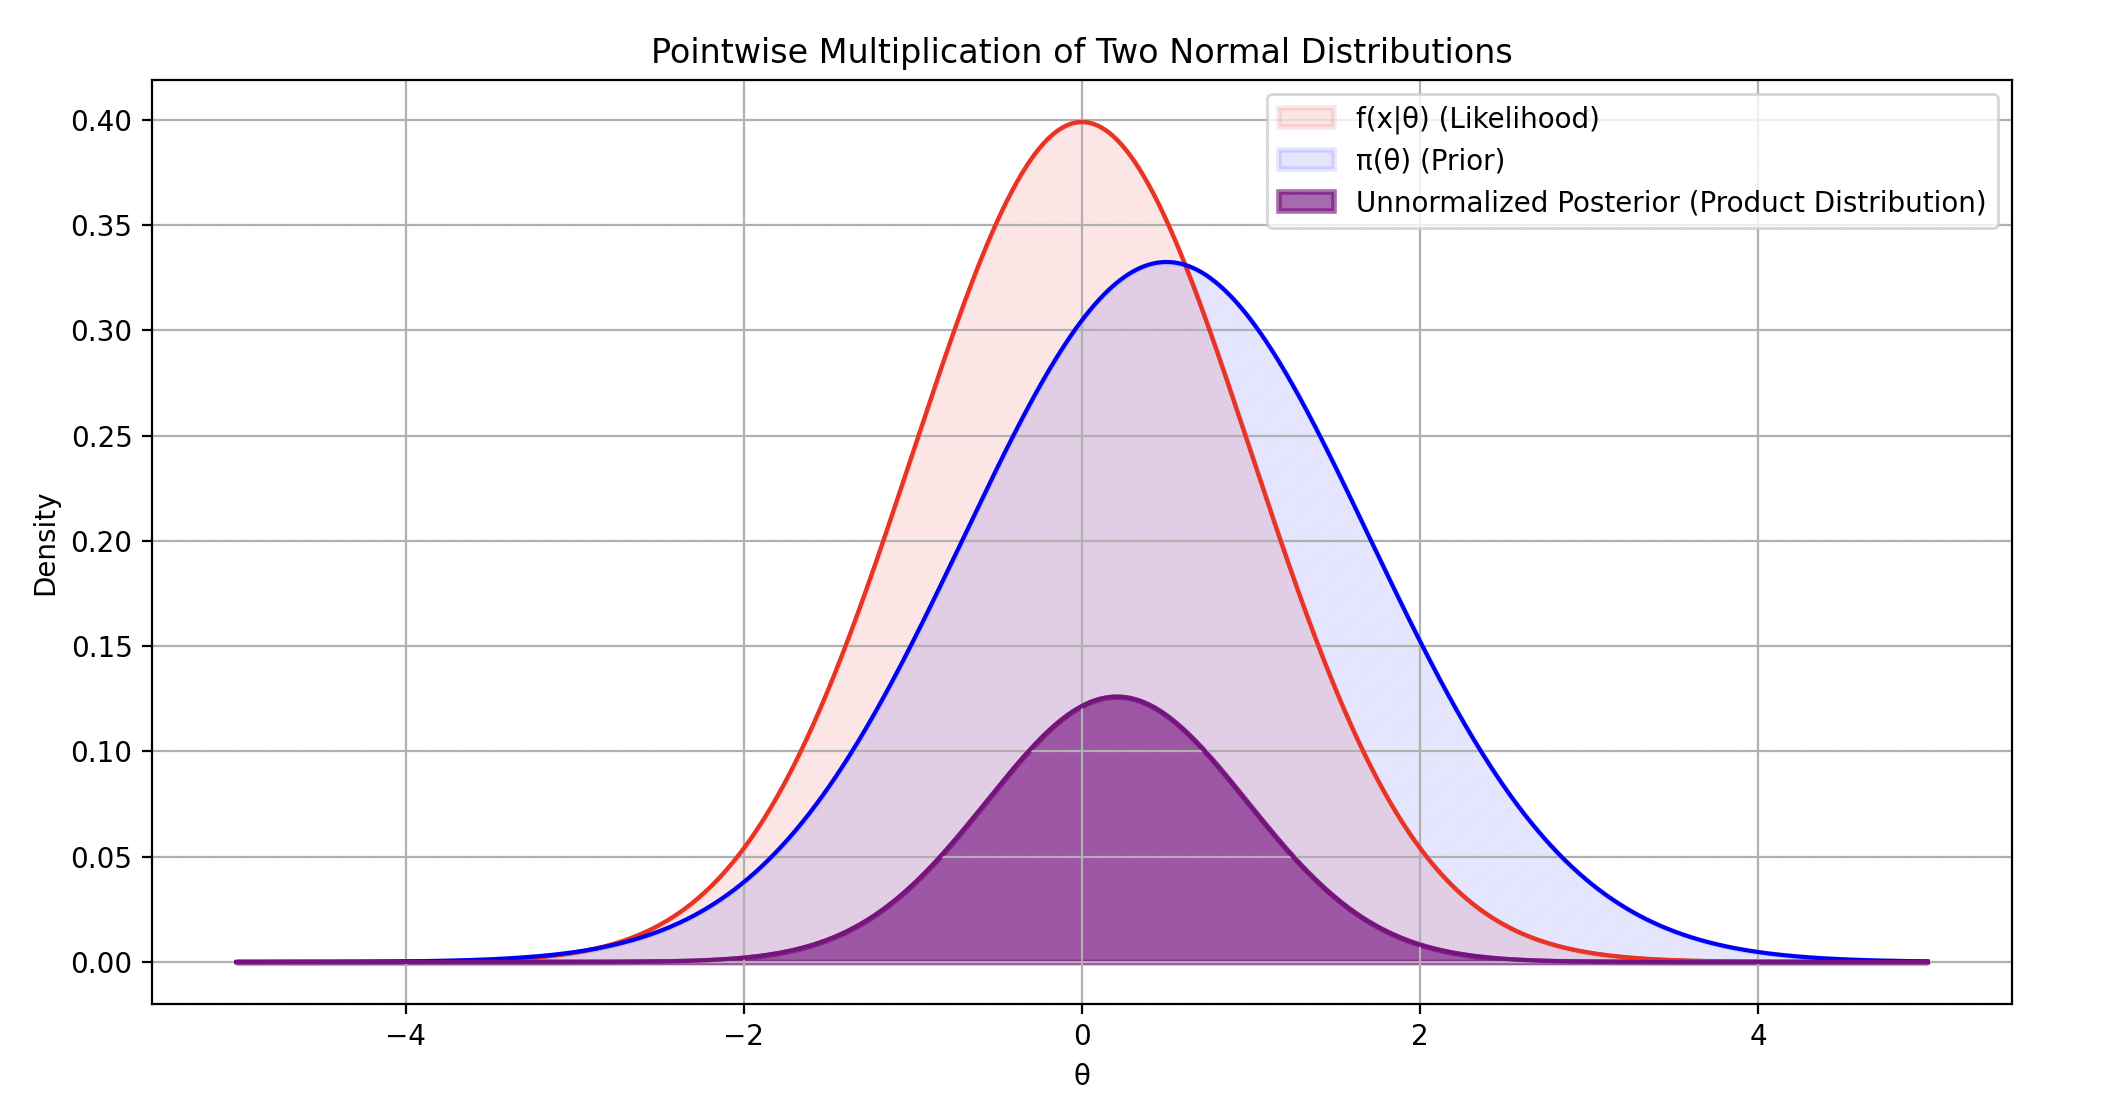
\includegraphics[width=1.0\textwidth]{assets/visual_8.png} 
\caption{Two factor distributions and their product distribution}
\label{fig:cond_prob}
\end{figure}

\noindent It's worth taking a moment to understand what the representation above expresses. As shown, the product distribution appears to be centered between the hypothetical likelihood and prior distributions. This distribution positioning represents the idea that the product distribution is indeed accounting for information from both experiment (likelihood) and prior beliefs. The two distributions are multiplied together by an operation called a point-wise multiplication. A point-wise multiplication of two distributions involves multiplying the values of their representative functions at each point in their domain, resulting in a new distribution that reflects the combined characteristics of both original distributions at each point. This process is visually demonstrated for a discrete case below:

% Image
\begin{figure}[h!]
\centering
\includegraphics[width=1.0\textwidth]{assets/visual_9.png} 
\caption{Point-wise multiplication visualized for a discrete case}
\label{fig:cond_prob}
\end{figure}

\subsection*{The Posterior}
\noindent While the product distribution clearly incorporates data from both prior beliefs and experiment, its evident that the product distribution's total area is significantly smaller than both of the factor distributions. This is a problem, as the distribution must integrate to 1 in order to be considered a valid probability distribution. At this moment, the product distribution is proportional to what will be the posterior distribution $\pi(\theta \mid x)$, but it does not integrate to 1. For that reason, it's called the \textit{unnormalized posterior}. To obtain a valid posterior probability distribution, we need a distribution that achieves the following two properties: first, it must be proportional to the unnormalized posterior distribution and second, it must integrate to 1. To achieve these properties, the unnormalized posterior can be divided by what's called the\textit{normalizing constant}, which is the scalar value, $\int_{\Theta} f(x \mid \theta) \pi(\theta) d\theta$.\\


\subsection*{The Normalizing Constant}
\noindent The following offers an algebraic explanation for why normalization requires dividing by the integral of the unnormalized posterior distribution function. Suppose we're given a function, $g(x)$ that we'd like to normalize to $f(x)$. Normalization requires that $f(x)$ satisfies the following:

\begin{equation}
\int_{-\infty}^{\infty} f(x) \, dx = 1
\end{equation}
\begin{equation}
f(x) \propto g(x) \implies f(x) = k g(x)
\end{equation}

\noindent Here, $k$ is the unknown normalizing constant. It can be found by substituting $kg(x)$ for $f(x)$ in equation 22,

\begin{equation}
\int_{-\infty}^{\infty} kg(x) \, dx = 1
\end{equation}
\begin{equation}
k\int_{-\infty}^{\infty} g(x) \, dx = 1
\end{equation}
\begin{equation}
\int_{-\infty}^{\infty} g(x) \, dx = \frac{1}{k}
\end{equation}
\begin{equation}
k = \frac{1}{\int_{-\infty}^{\infty} g(x) \, dx}
\end{equation}
\begin{equation}
\implies f(x) = \frac{g(x)}{\int_{-\infty}^{\infty} g(x) \, dx}
\end{equation}

\noindent As expected, integrating $f(x)$ yields 1, satisfying equation 22.
\begin{equation}
\int_{-\infty}^{\infty} f(x)\, dx = \frac{\int_{-\infty}^{\infty} g(x) \, dx}{\int_{-\infty}^{\infty} g(x) \, dx} = 1
\end{equation}

\noindent This concludes the normalization of $g(x)$. In practice, the normalizing constant may be difficult to compute, which gives rise to probabilistic sampling methods, such as the Metropolis-Hastings and Gibbs Sampling algorithms.


\subsection*{Conclusion}
\noindent It is my hope that this document serves as a useful tool for better understanding some of the mechanics involved in Bayes' Theorem. As a fan of open-source software, the Latex for this document will be available on GitHub. If anything is incorrect or can be better explained, I strongly urge you to open a pull request! Thank you.

\end{document}

